\section{Convolutional Neural Network}
\label{sec:cnn}
\subsection{Hyperparameter Optimization}

\subsubsection{Convolutional Layers}

Convolutional layers are the core of the \gls{cnn} architecture by harnessing three key concepts—sparse interactions,
parameter sharing, and spatially equivariant feature representations—that collectively contribute to a robust and efficient
component for feature extraction~\cite[Chapter 9]{dlbook}. \\
These layers employ multiple kernels (\( \coloneqq \) filters) that extend across all channels of the input data and perform
a convolution through the spatial dimension of the input sequence. \\
Our input data to the one-dimensional convolutional layers (\texttt{nn.Conv1d}) can be perceived as a
sequence of eigenvalues with length \(  L_{\text{seq}} = M \), exhibiting a single channel \( C_{\text{in}} = 1\), or
as a singleton sequence with \( C_{\text{in}} = M \) channels. \\
Each filter produces a feature map, representing the presence of specific patterns detected in the input, with the number
of output channels in a convolutional layer corresponding to the number of these finite impulse response filters.

\textbf{The Number of Channels} presents a critical hyperparameter that dominates the model's capacity for feature detection.

\begin{figure}[H]
    \centering
    \subfloat[]{{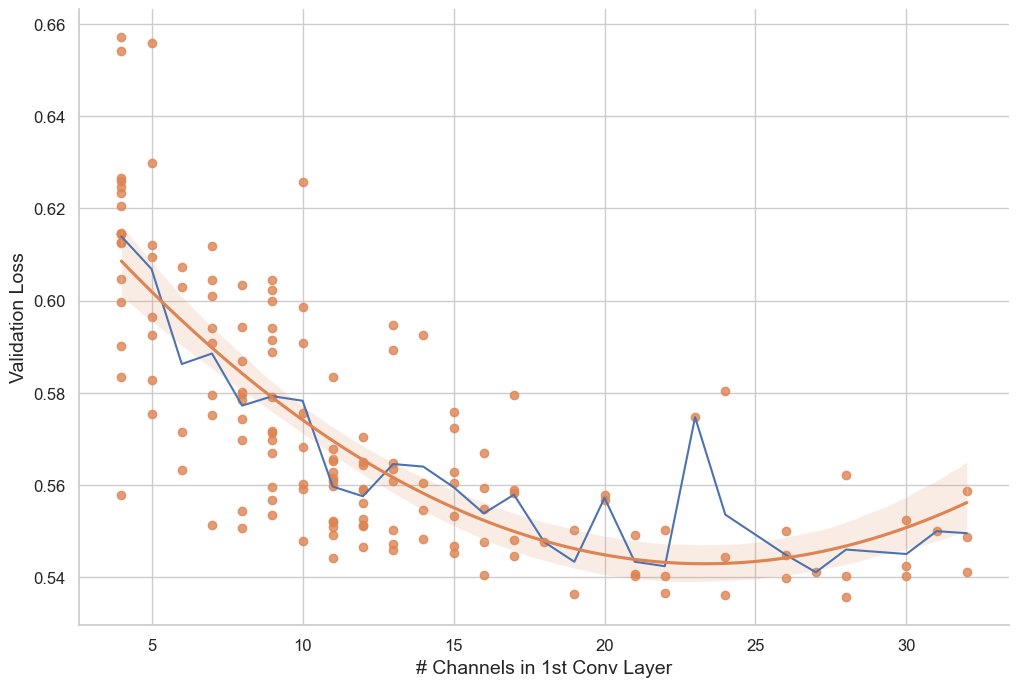
\includegraphics[width=0.48\textwidth]{figures/06_ModelExploration/4_CNN/conv_ch1.png}}}
    \subfloat[]{{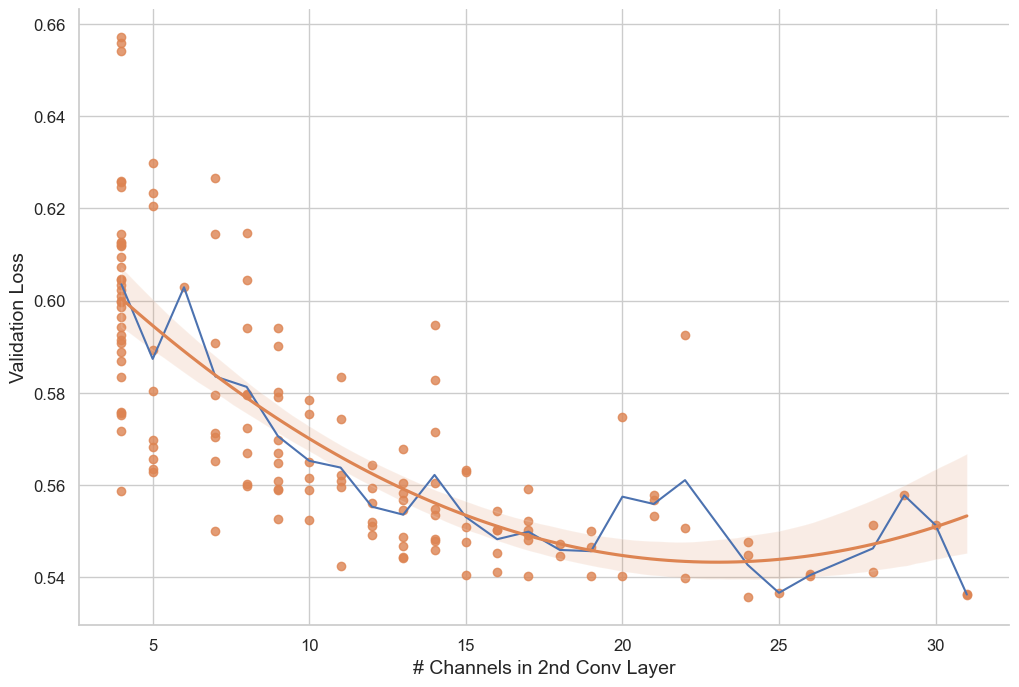
\includegraphics[width=0.48\textwidth]{figures/06_ModelExploration/4_CNN/conv_ch2.png}}}
    \caption{Influence of the number of channels in the first (a) and second (b) convolutional layers on \( \lossCEVal \).}
    \label{fig:ch1ch2}
\end{figure}

\begin{figure}[H]
    \centering
    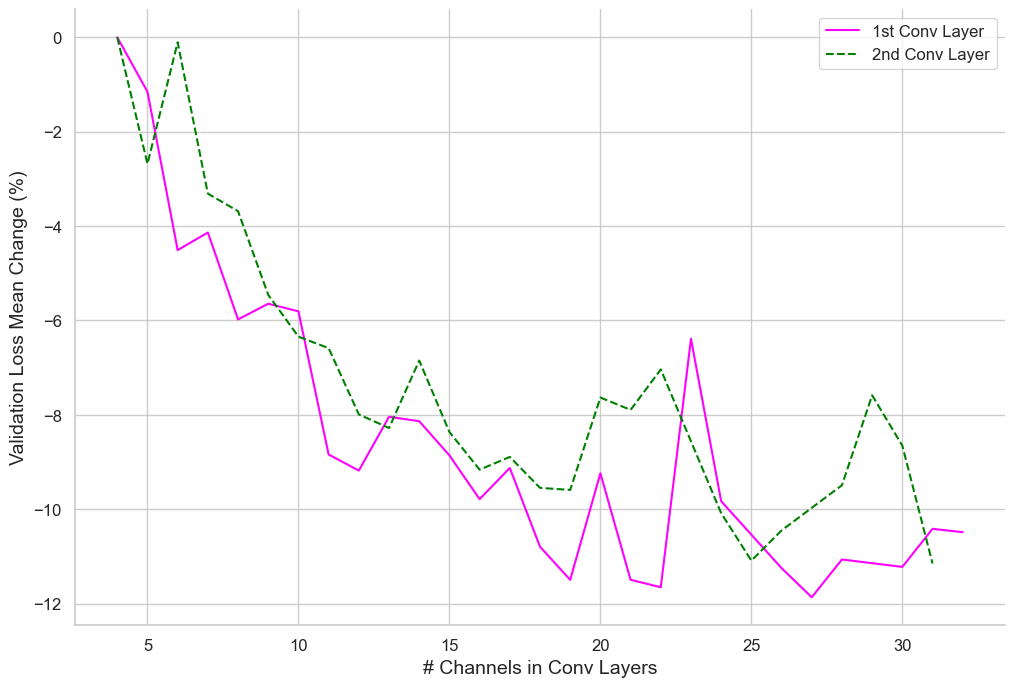
\includegraphics[width=0.5\textwidth]{figures/06_ModelExploration/4_CNN/conv_ch_change.png}
    \caption{Relative changes in validation loss for varying number of channels in both conv blocks.}
    \label{fig:ch1ch2_relchange}
\end{figure}

Figures~\ref{fig:ch1ch2} and~\ref{fig:ch1ch2_relchange} illustrate how varying the number of channels affects model
performance, guiding the selection towards an optimal balance that maximizes feature extraction while minimizing the
likelihood of overfitting.\\
Both figures indicate that the explored ranges of channels \( C_{\text{out}} \) were chosen appropriately, given that
the validation loss \( \lossCEVal \) exibits a local minimum, beyond which the loss increases due to overfitting. \\

\textbf{Pooling Layers} complement convolutional layers by reducing the spatial dimension of the feature maps,
thus allowing the model to capture higher-level features with a greater local dispersion. \\

The sizes of the pooling windows as well as other hyperparameters which are linked to the convolutional layers, all have
an impact on the model's performance, as depicted in Figure~\ref{fig:param_impact}.

\begin{figure}[H]
    \centering
    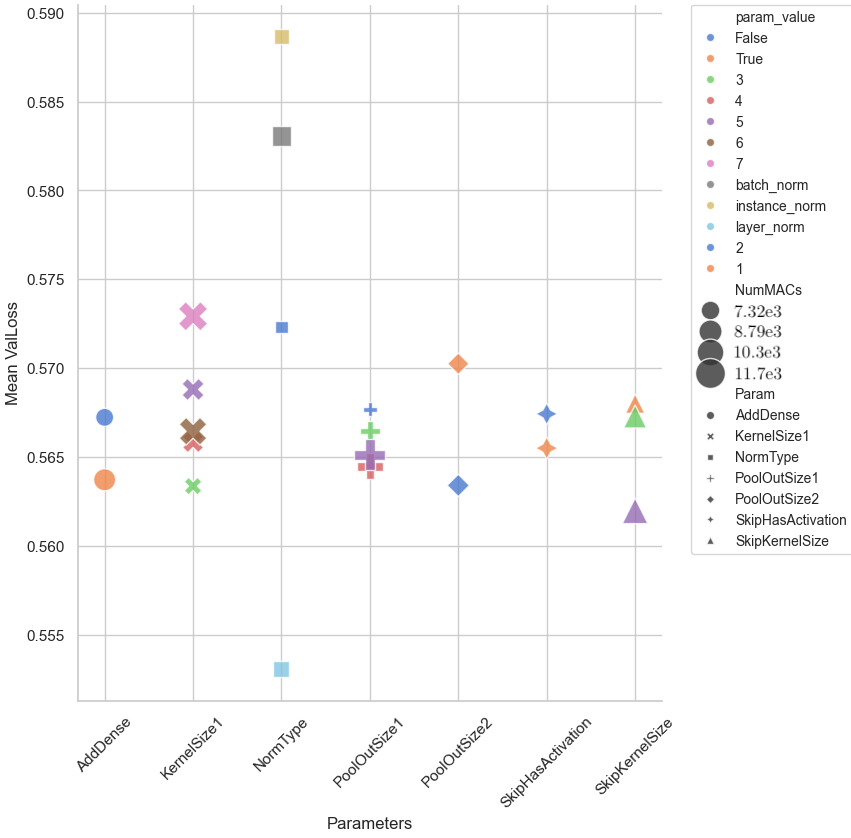
\includegraphics[width=0.6\textwidth]{figures/06_ModelExploration/4_CNN/scatter.png}
    \caption{Scatter plot showing the impact of different hyperparameters on mean validation loss.}
    \label{fig:param_impact}
\end{figure}

Figure~\ref{fig:param_impact} presents a scatter plot of various hyperparameter configurations and their corresponding
mean validation loss. Each point represents a unique combination of parameters such as kernel size, normalization type,
and pooling size. The plot indicates the sensitivities of the validation loss to these hyperparameters, with certain
configurations leading to lower loss values and thus better model performance.

The scatter plot also highlights the trade-offs between model complexity, as indicated by the size of the points
representing the number of \glspl{mac}.\\
For example, larger kernels and additional dense layers may contribute
to a lower validation loss but also increase the computational requirements. Conversely, smaller kernels and fewer dense
layers might yield a less complex model but potentially at the cost of higher validation loss.

The other depicted criteria, such as the type of normalization layer, will be discussed subsequently.

\subsubsection{Normalization Layers}
Normalization layers, crucial for modern deep networks, standardize the activations of each layer,
thus enhancing the optimization process and the network's generalization capabilities. \\
Even in shallow networks, normalization proves beneficial, as it stabilizes the gradient flow by reducing the sharpness
of the loss surface. \\
A smoother loss surface is associated with a reduced risk of overfitting since it is less likely
to contain sharp local minima, which are more prone to overfitting and generally hinder the optimization process~\cite{lyu2023norm}.\\
Another advantage is the reduction of the internal covariate shift, which is the change in the distribution of network's activations during training, as
well as the consequent potential for faster convergence through the employment of larger learning rates. \\

In the context of this work, three normalization layers were considered: Batch Normalization, Instance Normalization,
and Layer Normalization, each visualized in~\autoref{fig:all_norm_types}.

\begin{figure}[H]
    \centering
    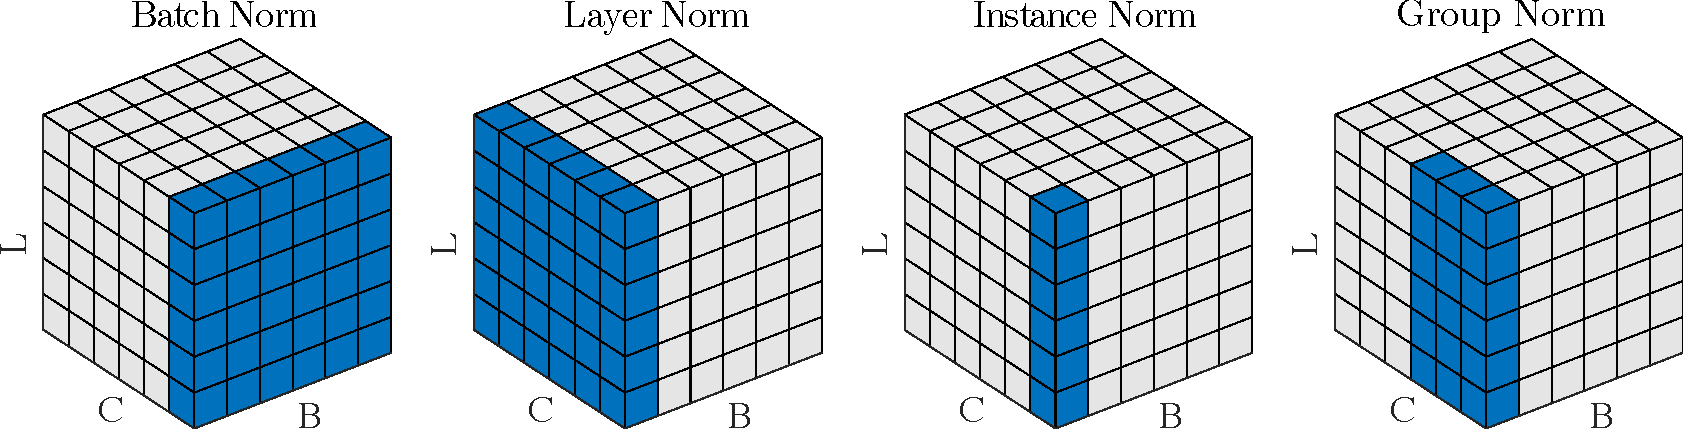
\includegraphics[width=0.6\textwidth]{figures/06_ModelExploration/4_CNN/all_norms.pdf}
    \caption{Feature map tensors -- blue units are normalized by the same mean and variance~\cite{wu2018group}.}
    \label{fig:all_norm_types}
\end{figure}

Although, Group Normalization was not considered in this work, it is worth mentioning it, since it was shown to outperform
the other normalization layers in the context of small batch sizes~\cite{wu2018group}, while being on par with Group Norm for larger batch
sizes, while exhibiting no dependence on the batch size. \\
Batch Normalization computes statistics (\(\mathbb{E}[\bfm{X}], \operatorname{Var}[\bfm{X}]\)) across the spatial
dimensions and all samples in the mini-batch for each channel, Layer Normalization along the \((L, C)\) axes for each
sample, and Instance Normalization along the \(L\) axis for each sample and channel~\cite{wu2018group}.

They all aim to compensate for the possible loss of representational capacity by introducing a learnable linear
transformation, parametrized by \( \bfm{\gamma} \) and \( \bfm{\beta} \),
that scales and shifts the normalized value~\cite{wu2018group}, expressed for Layer Normalization as~\cite{PyTorchLayerNorm}:
\begin{equation}
    \bfm{Y}_{b, :, :} = \bfm{\gamma} \odot \left( \frac{\bfm{X}_{b, :, :} - \mathrm{E}[\bfm{X}_{b, :, :}]}{\sqrt{\operatorname{Var}[\bfm{X}_{b, :, :}] + \epsilon}} \right) + \bfm{\beta}, \quad \text { where } \bfm{\gamma}, \bfm{\beta} \in \mathbb{R}^{C \times L}
\end{equation}

The validation loss for each normalization layer is depicted in~\autoref{fig:norm_type}.
\begin{figure}[H]
    \centering
    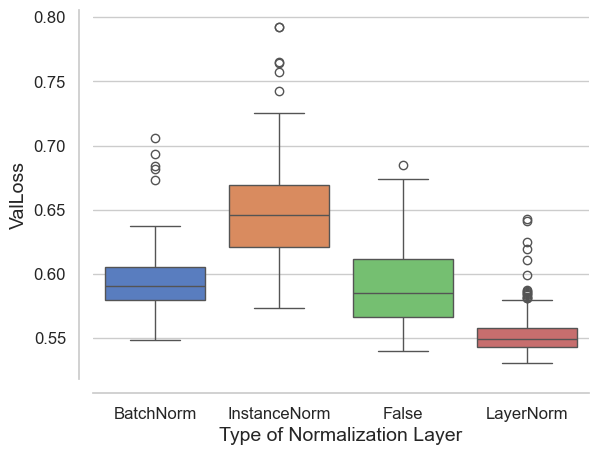
\includegraphics[width=0.6\textwidth]{figures/06_ModelExploration/4_CNN/conv_norm_type.png}
    \caption{Validation loss for different normalization layers.}
    \label{fig:norm_type}
\end{figure}

As shown in~\autoref{fig:norm_type}, the application of layer normalization (Layer Norm) resulted in the lowest \( \meanLossCEVal \),
while Instance Norm and Batch Norm performed worse. The respective layer's impacts on the model's performance and complexity
are summarized in~\autoref{tab:norm_type}.

\begin{table}[H]
    \centering
    \caption{Comparison of different normalization layers and their effects on mean validation loss and model complexity.}
    \label{tab:norm_type}
    \begin{tabular}{@{}lcccccccc@{}}
    \toprule
    & \multicolumn{2}{c}{\( \meanLossCEVal \) } & \multicolumn{2}{c}{\( \meanAccVal \)} & \multicolumn{2}{c}{\#Params} & \multicolumn{2}{c}{\#MACs} \\
    \cmidrule(lr){2-3} \cmidrule(lr){4-5} \cmidrule(lr){6-7} \cmidrule(lr){8-9}
    Normalization & \( \nu \) & \( \%\Delta \) & \( \nu \) & \( \%\Delta \) & \( \nu \) & \( \%\Delta \) & \( \nu \) & \( \%\Delta \) \\
    \midrule
    None               & 0.590 & —            & 0.737 & —            & 2322 & —    & 7.01e3 & — \\
    Batch Norm          & 0.596 & \rdbx{+0.98\%} & 0.732 & \rdbx{-0.573\%} & 2787 & \rdbx{+20.0\%} & 10.7e3 & \rdbx{+53.6\%} \\
    Instance Norm       & 0.648 & \rdbx{+9.91\%} & 0.712 & \rdbx{-3.31\%}  & 2858 & \rdbx{+23.1\%} & 10.6e3 & \rdbx{+52.3\%} \\
    Layer Norm          & 0.553 & \gnbx{-6.16\%} & 0.748 & \gnbx{+1.61\%}  & 3414 & \rdbx{+47.0\%} & 9.52e3 & \rdbx{+35.8\%} \\
    \bottomrule
    \end{tabular}
\end{table}


The underwheling performance of Instance Norm is likely due its inherent unsuitablity for the task at hand, given that
it was originally designed for style transfer and image generation tasks and generally requires larger spatial or temporal
dimensions to effectively estimate the mean and variance of the input data.
Moreover, Instance Norm was \emph{not} implemented with the subsequent affine transformation, which also contributed to its
underperformance.\\
Layer Norm has demonstrated its capability to address various shortcomings of Batch Norm~\cite{ba2016layer}, although
such shortcomings were not expected to be significant in this context.

Surprisingly, Batch Norm's performance was not as strong as anticipated, despite its common application in \gls{cnn} architectures
and the use of a relatively large batch size \( \B = 1024 \). The most likely explanation is that the optimization process
was conducted with a dropout rate of eight percent in each convolutional block.
Since both Batch Norm and Dropout layers introduce noise to the optimization process, their combined use could have
hindered optimal convergence. \\
It would be worthwhile to investigate Batch Norm's performance without the inclusion of dropout layers, as it is
hypothesized to surpass Layer Norm's performance when considering the large batch size~\cite{wu2018group}.


Layer Norm distinguished itself among the normalization techniques evaluated, offering superior model performance and lower complexity. \\
The advantage of Layer Norm over Batch Norm, in terms of the number of \glspl{mac}, seems paradoxical.
Batch Norm separates the entire mini-batch into \( C \) independent normalization groups, whereas Layer Norm normalizes
each sample independently. Considering that \( \B \gg C \), and \( \text{\#Params}_{\text{LN}} = L \cdot \text{\#Params}_{\text{BN}} \),
this result appears counterintuitive. \\



\subsubsection{Activation Function}
Activation functions play a critical role in neural networks, introducing non-linear properties to the system,
which allows the model to learn complex non-linear patterns in the data. The choice of activation function can
significantly affect the learning dynamics and performance of the network.

Traditionally, the \gls{relu} has been widely used due to its simplicity, effectiveness in addressing the vanishing
gradient problem, and its advantageous effects on the convergence of the optimization process over activation functions that
introduce non-zero second derivatives~\cite[Chapter 6.3.1]{dlbook}.\\
However, \gls{relu} can introduce ``dead units'', which are neurons that never activate, and therefore bring no contribution
to the network's discriminative and predictive capabilities.\\
To overcome this, variations like leaky \gls{relu}, \gls{prelu} and \gls{elu} have been proposed, which allow a small,
positive gradient for negative input values, thus preventing the issue of dead units and allowing higher learning rates~\cite{dyingRelu}.

The equations defining each activation function are as follows:

\begin{align}
    \texttt{ReLU}(x) &= \max(0, x) \label{eq:relu} \\
    \texttt{PReLU}(x) &= \begin{cases}
        x & \text{if } x > 0 \\
        \alpha x & \text{if } x \leq 0
    \end{cases}, \quad \text{where } \alpha \text{ is a learnable parameter} \label{eq:prelu} \\
    \texttt{ELU}(x) &= \begin{cases}
        x & \text{if } x > 0 \\
        \alpha \left( e^x - 1 \right) & \text{if } x \leq 0
    \end{cases}, \quad \text{where } \alpha = 1 \text{ per default}\label{eq:elu}
\end{align}

\begin{figure}[H]
    \centering
    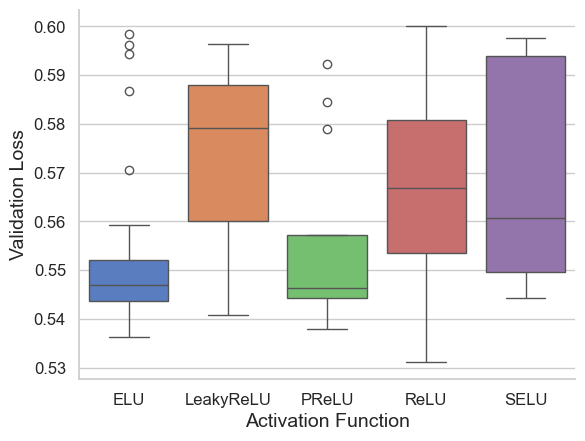
\includegraphics[width=0.55\textwidth]{figures/06_ModelExploration/4_CNN/activ_fn.png}
    \caption{Boxplots of \( \lossCEVal \) for different activation functions.}
    \label{fig:activ_fn}
\end{figure}

\autoref{fig:activ_fn} demonstrates the influence of activation functions on model performance through the distribution
of validation loss. Among the evaluated functions, \gls{prelu} and \gls{elu} show a slight advantage over \gls{relu} in terms of validation
loss, indicating potential improvements in learning dynamics and model robustness. \\
The advantages of \gls{prelu} and \gls{elu} over \gls{relu} are further quantified in \autoref{tab:activation_fn}.

\begin{table}[H]
    \centering
    \caption{Comparison of Validation Loss for Different Activation Functions}
    \label{tab:activation_fn}
    \begin{tabular}{@{}lcc@{}}
    \toprule
    Activation Function & \multicolumn{2}{c}{\( \meanLossCEVal \) } \\
    \cmidrule(lr){2-3}
                      & \( \nu \) & \( \%\Delta \) \\
    \midrule
    \gls{relu}    & 0.567 & —           \\
    \gls{prelu}   & 0.555 & \gnbx{-2.10} \\
    \gls{elu}     & 0.551 & \gnbx{-2.69} \\
    \bottomrule
    \end{tabular}
\end{table}

\gls{elu}'s smoother transition from negative to positive inputs theoretically benefits learning dynamics but
comes at a higher computational cost due to the exponential function, which might be disadvantageous for deployment on resource-constrained platforms like \glspl{fpga}.
Conversely, \gls{prelu} offers a compromise by introducing a learnable parameter, \( \alpha \), that adjusts the slope for negative inputs, offering flexibility without
significantly increasing computational demands. For this reason, \gls{prelu}, with a single shared \(\alpha\) parameter across
channels, is chosen for its balance between performance improvement and computational efficiency.
This consideration ensures that the selected activation function optimizes learning while remaining feasible for deployment
on resource-constrained platforms.

\subsubsection{The Resulting CNNP Block}
\label{subsubsec:cnn_block}

The construction of the \texttt{CNNP} block represents a synthesis of empirical findings from the exploratory process
and theoretical considerations, yielding a composite layer structure within the convolutional neural network framework.

It comprises a sequential arrangement of a one-dimensional convolutional layer (\texttt{nn.Conv1d}), followed by a
layer normalization module (\texttt{nn.LayerNorm}), a parametric rectified linear unit (\texttt{nn.PReLU}), and an
adaptive max pooling layer (\texttt{nn.AdaptiveMaxPool1d}), concluding with a dropout layer to mitigate overfitting.

\[
    \texttt{CNNP} \coloneqq \underbrace{\texttt{nn.Conv1d}}_{\text{\textbf{C}onv}}
    \rightarrow \underbrace{\texttt{nn.Layer Norm}}_{\text{\textbf{N}orm}}
    \rightarrow \underbrace{\texttt{nn.PReLU}}_{\text{\textbf{N}on-linear}}
    \rightarrow \underbrace{\texttt{nn.AdaptiveMaxPool1d}}_{\text{\textbf{P}ool}}
    \rightarrow \texttt{nn.Dropout}
\]

The dropout rate was optimized parallel to the other hyperparameters, depicted in~\autoref{fig:param_impact}, and its
impact on the model's performance can be found in the appendix~\autoref{fig:dropout_cnn}.


\subsubsection{Skip Connection}

Skip connections, are a fundamental architectural feature in deep neural networks that enable the training of significantly
deeper models by providing advantageous optimization trajectories through the loss landscape or allowing for the reuse or
preservation of important features throughout the network. \\
The most prominent example of a skip connection is the residual connection, which was first introduced in the ResNet architecture~\cite{he2015deep}.
Residual connections aim to address the degradation problem, which is the phenomenon where increasing the depth of a network
results in higher training error due to various optimization difficulties. \\
The application of residual connections mostly aims to achieve better optimization dynamics by reformulating the
bypassed layers' training objectives to learn the residual (\( \coloneq \) difference) from the identity mapping, instead
of learning an unreferenced mapping from scratch.

Since the phenomenon of degradation is more prevalent in very deep networks, which might be up to 2 orders of magnitude deeper
than our model, the use of skip connections is not motivated by the degradation problem, but rather by the goal to allow
for more diverse feature representations.
The use of skip connections in our model architecture is motivated by the
desire to create an ensemble of the two parallel paths, which can be seen as an ensemble of the serially connected
\texttt(CNNP)s and a layer that performs the operation formalized in~\autoref{eq:skip_connection}.
\begin{equation}
    \bfm{X}_{:, j}^{\text{(skip)}} = \texttt{ReLU}\left(\text{bias}_j + \sum_{k=0}^{M} \bfLT_{:, k, 1}^P \cdot W_{jk}\right), \quad  \bfm{X}^{\text{(skip)}} \in \mathbb{R}^{\B \times C_{\text{out}}^{(\text{skip})}}, \: j = 1, \ldots, C_{\text{out}}^{(\text{skip})}
    \label{eq:skip_connection}
\end{equation}
The input to the skip connection is the permuted tensor of eigenvalues \( \bfLT^P \coloneqq \texttt{permute}( \bfLT, [0, 2, 1] ) \).
\( C_{\text{in}}^{(\text{skip})} = M = \| \bfL \| \) is the number of input channels, \( C_{\text{out}}^{(\text{skip})} \)
is the number of output channels, and \( \bfm{W} \) are the weights of the \( 1 \times 1 \) convolutional layer in the
skip connection.

In contrast to a residual connection, the outputs of our skip connection \( \bfm{X}^{\text{(skip)}} \) are not
added to the outputs of the ``main'' path, but are concatenated to them. \\
Adding the outputs of the skip connection and the main path requires both operands to exhibit the same dimensions, which is
not the case in our model architecture. Moreover, concatenation preserves a more diverse feature representation since
it allows both paths to learn different features, rather than simplifying the learning task by allowing the model to
learn the residual from the identity mapping. \\

\begin{table}[H]
    \centering
    \caption{Comparison of model performance with and without skip connections}
    \label{tab:residual_comparison}
    \begin{tabular}{@{}lcccccccc@{}}
    \toprule
    & \multicolumn{2}{c}{\( \meanLossCEVal \) } & \multicolumn{2}{c}{\( \meanAccVal \)} & \multicolumn{2}{c}{\#Params} & \multicolumn{2}{c}{\#MACs} \\
    \cmidrule(lr){2-3} \cmidrule(lr){4-5} \cmidrule(lr){6-7} \cmidrule(lr){8-9}3
    Skip Connection & \( \nu \) & \( \%\Delta \) & \( \nu \) & \( \%\Delta \) & \( \nu \) & \( \%\Delta \) & \( \nu \) & \( \%\Delta \) \\
    \midrule
    None & 0.544 & - & 0.753 & - & 2667 & - & 8984 & - \\
    Skip & 0.545 & \rdbx{0.296} & 0.751 & \rdbx{-0.183} & 2721 & \rdbx{2.02} & 9038 & \rdbx{0.601} \\
    Skip \( \oplus \) Conv & 0.537 & \gnbx{-1.28} & 0.756 & \gnbx{0.435} & 2747 & \rdbx{3.00} & 9036 & \rdbx{0.568} \\
    \bottomrule
    \end{tabular}
\end{table}

\autoref{tab:residual_comparison} shows the comparison of model performance with and without the skip connection. The second
column ``Skip'' refers to a model, in which the output of the serially connected \texttt{CNNP} blocks is concatenated with
the original input tensor of eigenvalues.
The third column ``Skip \( \oplus \) Conv'' refers to the model with skip connections as introudced in~\autoref{eq:skip_connection},
and depicted in~\autoref{fig:cnn_architecture}.\\
\autoref{fig:ch_skip} shows the influence of the number of channels in the skip connection \( C_{\text{out}}^{(\text{skip})} \) on
the validation loss \( \lossCEVal \).

\begin{figure}[H]
    \centering
    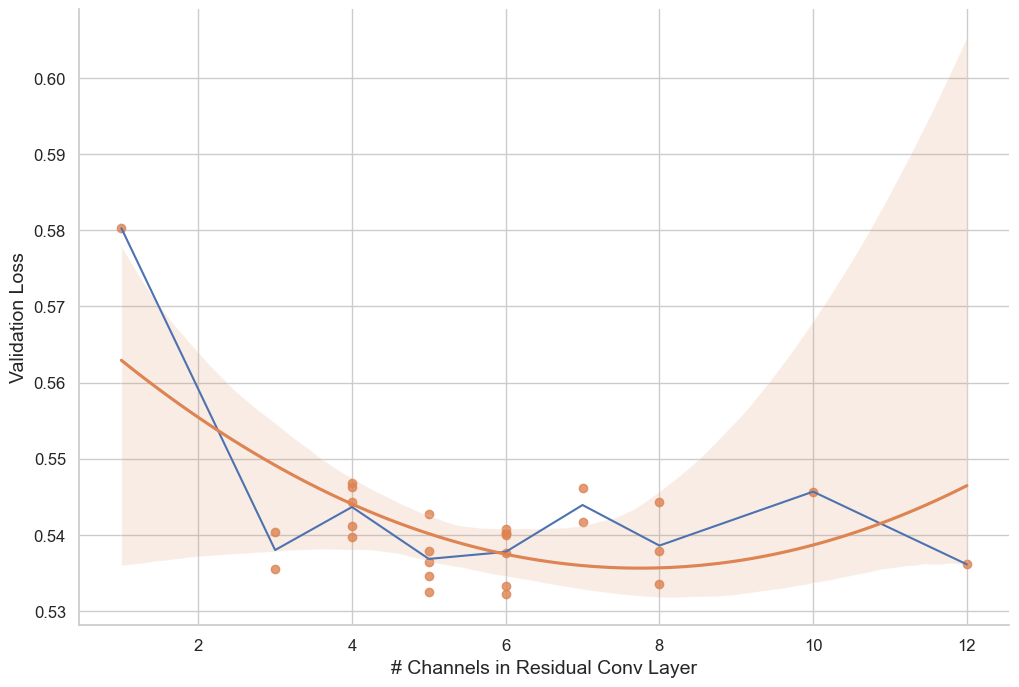
\includegraphics[width=0.45\textwidth]{figures/06_ModelExploration/4_CNN/conv_chskip.png}
    \caption{Influence of the number of channels in the skip connection.}
    \label{fig:ch_skip}
\end{figure}

Given the low number of optimization trials used to evaluate  \( C_{\text{out}}^{(\text{skip})} \), we decided to choose
a more conservative value of \( C_{\text{out}}^{(\text{skip})} = 5 \) to avoid overfitting. \\
Empirical evidence indicated a marginal performance increase when applying the \gls{relu} activation function to the
output of the skip connection. Its application post-concatenation introduces non-linearity that helps in the differentiation
and processing of features. Given its low
computational overhead and subtle positive impact on model performance, we decided to apply ReLU to our skip connections, thereby
leveraging the advantages of non-linearity while maintaining computational efficiency.

\paragraph{Varying Snapshot Count}
\hyperref[fig:cnn_plus_arch]{Figure~\ref*{fig:cnn_plus_arch}} conceptualizes the adaptation of the employed CNN architecture to handle a variable number
of snapshots by embedding the number of snapshots \( K \) into the skip branch of the network.
The results of the evaluation of the model with varying snapshot count will be presented in~\autoref{sec:influence_num_snapshots}.

\subsection{Resulting Architecture}
\label{subsubsec:resulting_architecture}

The development of the \gls{cnn} architecture, delineated in~\autoref{fig:cnn_architecture}, was achieved through a
methodical hyperparameter optimization facilitated by \textsc{Optuna}.
The optimization targeted a multidimensional objective function that accounted for validation loss (\( \meanLossCEVal \)),
model complexity (number of parameters and \glspl{mac}), and validation accuracy (\( \meanAccVal \)).

\begin{figure}[H]
    \centering
    \subfloat[]{{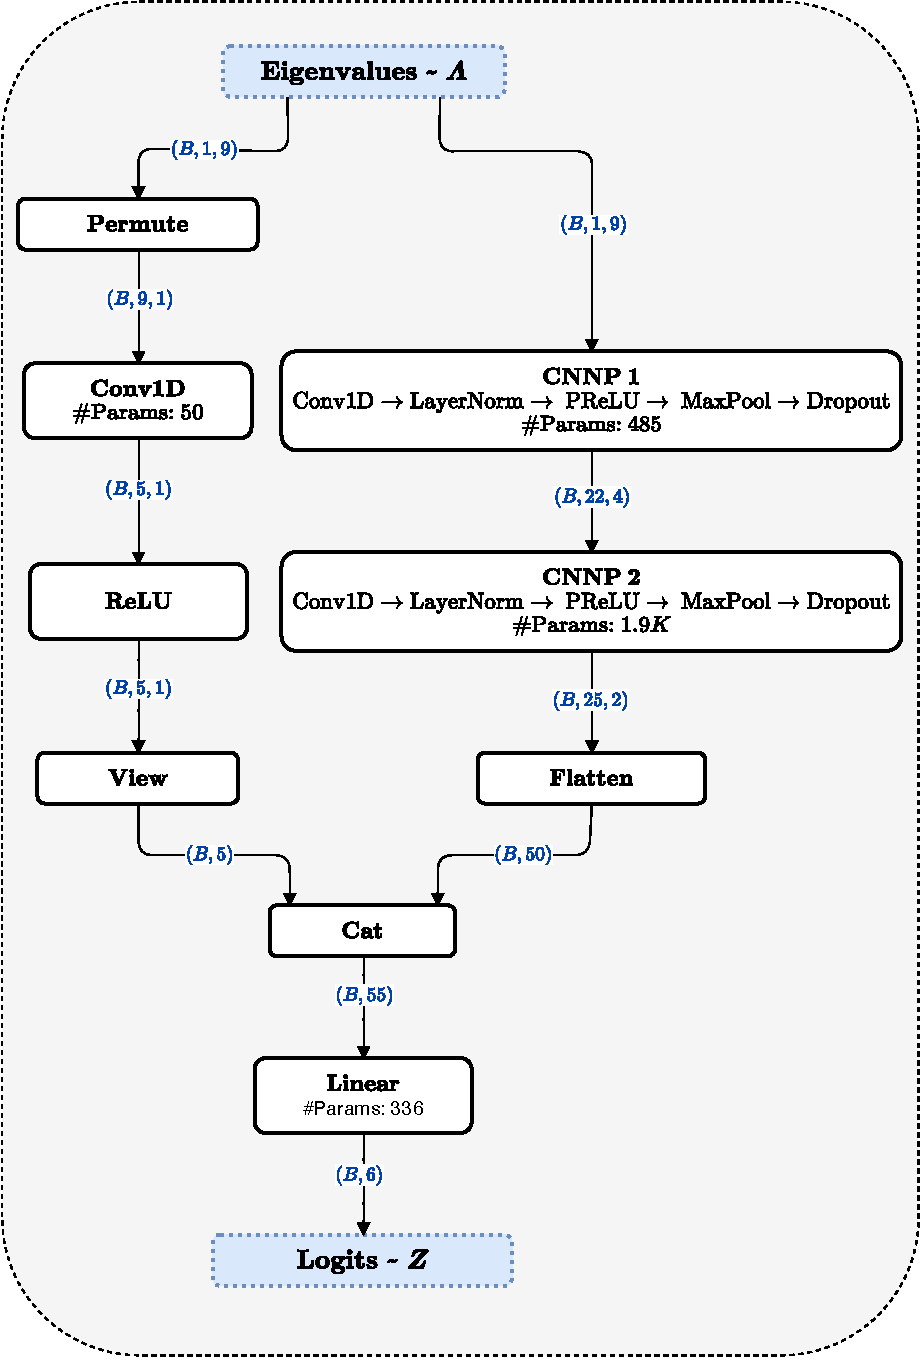
\includegraphics[width=0.41\textwidth]{figures/06_ModelExploration/4_CNN/cnn.pdf}}}
    \hspace{0.5cm}
    \subfloat[\label{fig:cnn_plus_arch}]{{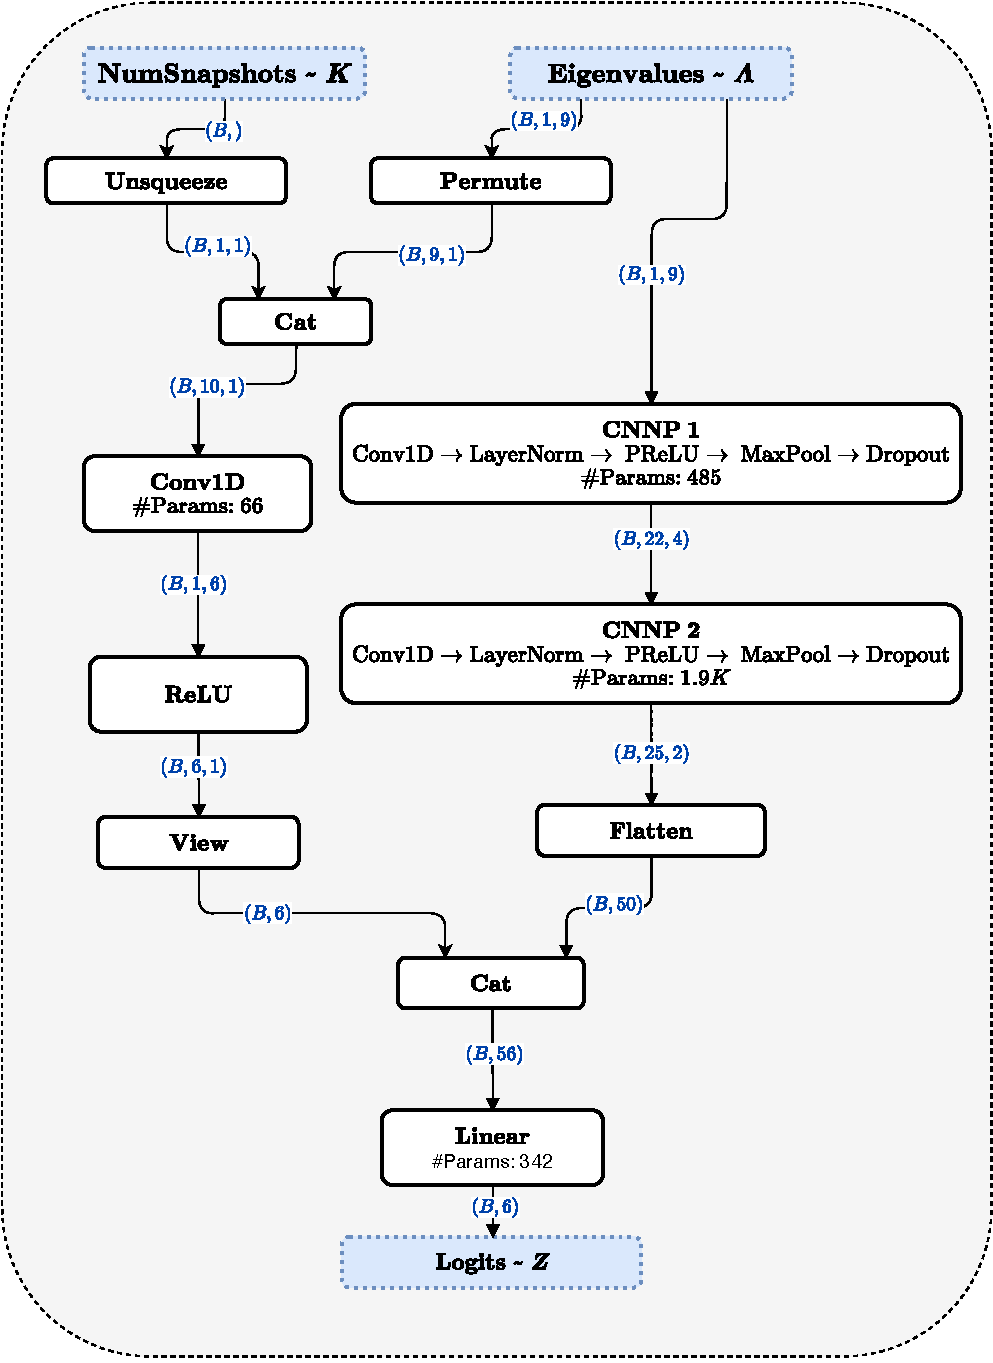
\includegraphics[width=0.44\textwidth]{figures/06_ModelExploration/4_CNN/cnn+.pdf}}}
    \caption{Schematic of the \gls{cnn} (a) and its variable snapshot adaptation (b).}
    \label{fig:cnn_architecture}
\end{figure}

The decision to employ a series connection of two \texttt{CNNP}'s in the ``main'' path can be attributed to the length
of the input sequence \( L_{\text{seq}} = M\), which is short enough, such that two \texttt{CNNP} blocks with kernel
sizes of three in combination with the adaptive max pooling%
\footnote{The dimensional reductions are denoted in~\autoref{tab:cnn_summary}}
layers can effectively capture relevant features at all spatial scales. \\
Experimental evaluations indicated that the addition of a third \texttt{CNNP} block without intermediate pooling did not
affect performance, while a singular \texttt{CNNP} block increased validation loss.

Detailed hyperparameters and layer configurations that underpin the network's structure and training methodology are
summarized in~\autoref{tab:cnn_summary}.

\begin{table}[H]
    \centering
    \caption{Summary of Hyperparameters and Layer Configurations}
    \label{tab:cnn_summary}
    \resizebox{\textwidth}{!}{%
    \begin{tabular}{@{}lll@{}}
    \textbf{Block / Module}               & \textbf{Child}        & \textbf{Parameters / Value}            \\ \midrule
    \multicolumn{3}{l}{\textbf{Modules}}                                                     \\ \midrule
    \multirow{7}{*}{\texttt{CNNP} Block 1}
                                         & \texttt{nn.Conv1d}           & Channels: \(1 \rightarrow 22\), Kernel Size: 3, Padding: \texttt{reflect} \\
                                         &                              & \#Params \( = C_{\text{in}} \times C_{\text{out}} \times k + C_{\text{out}} = 88\) \\
                                         & \texttt{nn.Layer Norm}        & \#Params \( = 2 \times C_{\text{out}} \times L_{\text{seq}} = 396 \) \\
                                         & \texttt{nn.PReLU}                & \#Params = 1            \\
                                         & \texttt{AdaptiveMaxPool1d}&  \(L_{\text{seq}} : 9 \rightarrow 4 \)                   \\
                                         & \texttt{nn.Dropout}          & Rate: 0.06                      \\
                                         & \( \Sigma \) \#Params                  &  \( 1 \times 22 \times 3 + 2 + 2 \times 22 \times 9 + 1 = 485 \)\\\midrule
    \multirow{7}{*}{\texttt{CNNP} Block 2}
                                         & \texttt{nn.Conv1d}           & Channels: \(22 \rightarrow 25\), Kernel Size: 3, Padding: \texttt{reflect} \\
                                         &                              & \#Params \( = C_{\text{in}} \times C_{\text{out}} \times k + C_{\text{out}} = 1675\) \\
                                         & \texttt{nn.Layer Norm}        & \#Params \( = 2 \times C_{\text{out}} \times L_{\text{seq}} = 200 \)                       \\
                                         & \texttt{nn.PReLU}                & \#Params = 1            \\
                                         & \texttt{nn.AdaptiveMaxPool1d}& \(L_{\text{seq}} : 4 \rightarrow 2 \)                   \\
                                         & \texttt{nn.Dropout}                   & Rate: 0.06                      \\
                                         & \( \Sigma \) \#Params                & \( 22 \times 25 \times 3 + 25 + 2 \times 25 \times 4 + 1 = 1876 \) \\\midrule
    \multirow{3}{*}{Skip Connection}     & \texttt{nn.Conv1d}          & Channels: \(9 \rightarrow 5\), Kernel Size: 1 \\
                                         &                              & \#Params \( = C_{\text{in}} \times C_{\text{out}} + C_{\text{out}} = 50 \) \\
                                         & \texttt{nn.ReLU}                &             \\ \midrule
    Head                                 & \texttt{nn.Linear}          & \#Params = \( (2 \times 25 + 5) \times \| \NSet \| + \| \NSet \| = 336 \) \\
    \midrule[0.1pt]
    \addlinespace[0.5cm]
    \( \Sigma \) \#Params                & \texttt{ConvNet8} & 2747 \\
    \bottomrule

    \addlinespace[1cm]
    \multicolumn{3}{l}{\textbf{Non-Layer Hyperparameters}}                                       \\ \midrule
    Optimizer                            &                           & \texttt{optim.AdamW} \\
    Batch Size                           &                           & 512                       \\
    Learning Rate                        &                           & 0.002                     \\
    Weight Decay                         &                           & 0.01685                   \\
    LR Scheduler                         &                           & \texttt{lr\_scheduler.ReduceLROnPlateau}\\
    Precision                            &                           & \texttt{32-true}     \\
    \bottomrule
    \end{tabular}%
    }
\end{table}

\autoref{tab:cnn_summary} presents the chosen hyperparameters, notably including the \texttt{AdamW} optimizer. \\
This optimizer modifies the \texttt{Adam} algorithm by applying weight decay directly to the model weights instead of
incorporating it into the gradient updates. This approach allows \texttt{AdamW} to achieve more effective regularization,
enhancing the model's generalization capabilities by decoupling weight decay from the learning rate's adaptive adjustments~\cite{loshchilov2019decoupled}.

While a batch size of 1024 was used during the optimization process, the final model was trained with a batch size of 512%
\footnote{A short optimization run yielded a batch size of \( \B = 504 \) as optimal value.},
as the latter yielded a lower validation loss. This can be attributed to the fact that lower batch sizes intorduce more noise
to the optimization process, which can be beneficial to escape sharp local minima, and thus improve the generalization capabilities.

Furthermore, we employed \texttt{ReduceLROnPlateau} as a learning rate scheduler.
A comparison with other suitable
learning rate schedulers, such as \texttt{CyclicLR}, \texttt{OneCycleLR}, and
\texttt{CosineAnnealingLR}, did not yield actionable insights, as the number of steps per epoch
was too high to effectively utilize any of these schedulers. \\
An effective way to overcome this issue will be introduced in~\autoref{subsub:training_data}.

The learning rate, weight decay and dropout rate have also been optimized. The results of this optimization process can
be found in the appendix -- see Figures~\ref{fig:dropout_cnn},~\ref{fig:lr_cnn}, and~\ref{fig:wd_cnn}. \\
The weight decay parameter was optimized solely for the \gls{cnn} and was uniformly applied to all yet to be introduced
models.

\newpage{}
